\begin{apendicesenv}

\partapendices


\printindex[urls]

\chapter{Protótipos iniciais do Tenho Dito}
\label{prototipos-apendice}

Foram desenvolvidos alguns protótipos de telas do sistema Tenho Dito, a ser desenvolvido nesse trabalho. Na tela inicial (figura \ref{tenhodito1}) será exibido um mapa político do Brasil e ao passar o \textit{mouse} pelos estados, o tema mais abordado pelos parlamentares que representam o estado é mostrado. Também existe a possibilidade de alterar a forma de visualização, além de ter uma abordagem por estado, o usuário pode escolher por partido ou por tema. Entretanto, a abordagem por tema não foi prototipada.

\begin{figure}[h]
  \centering
  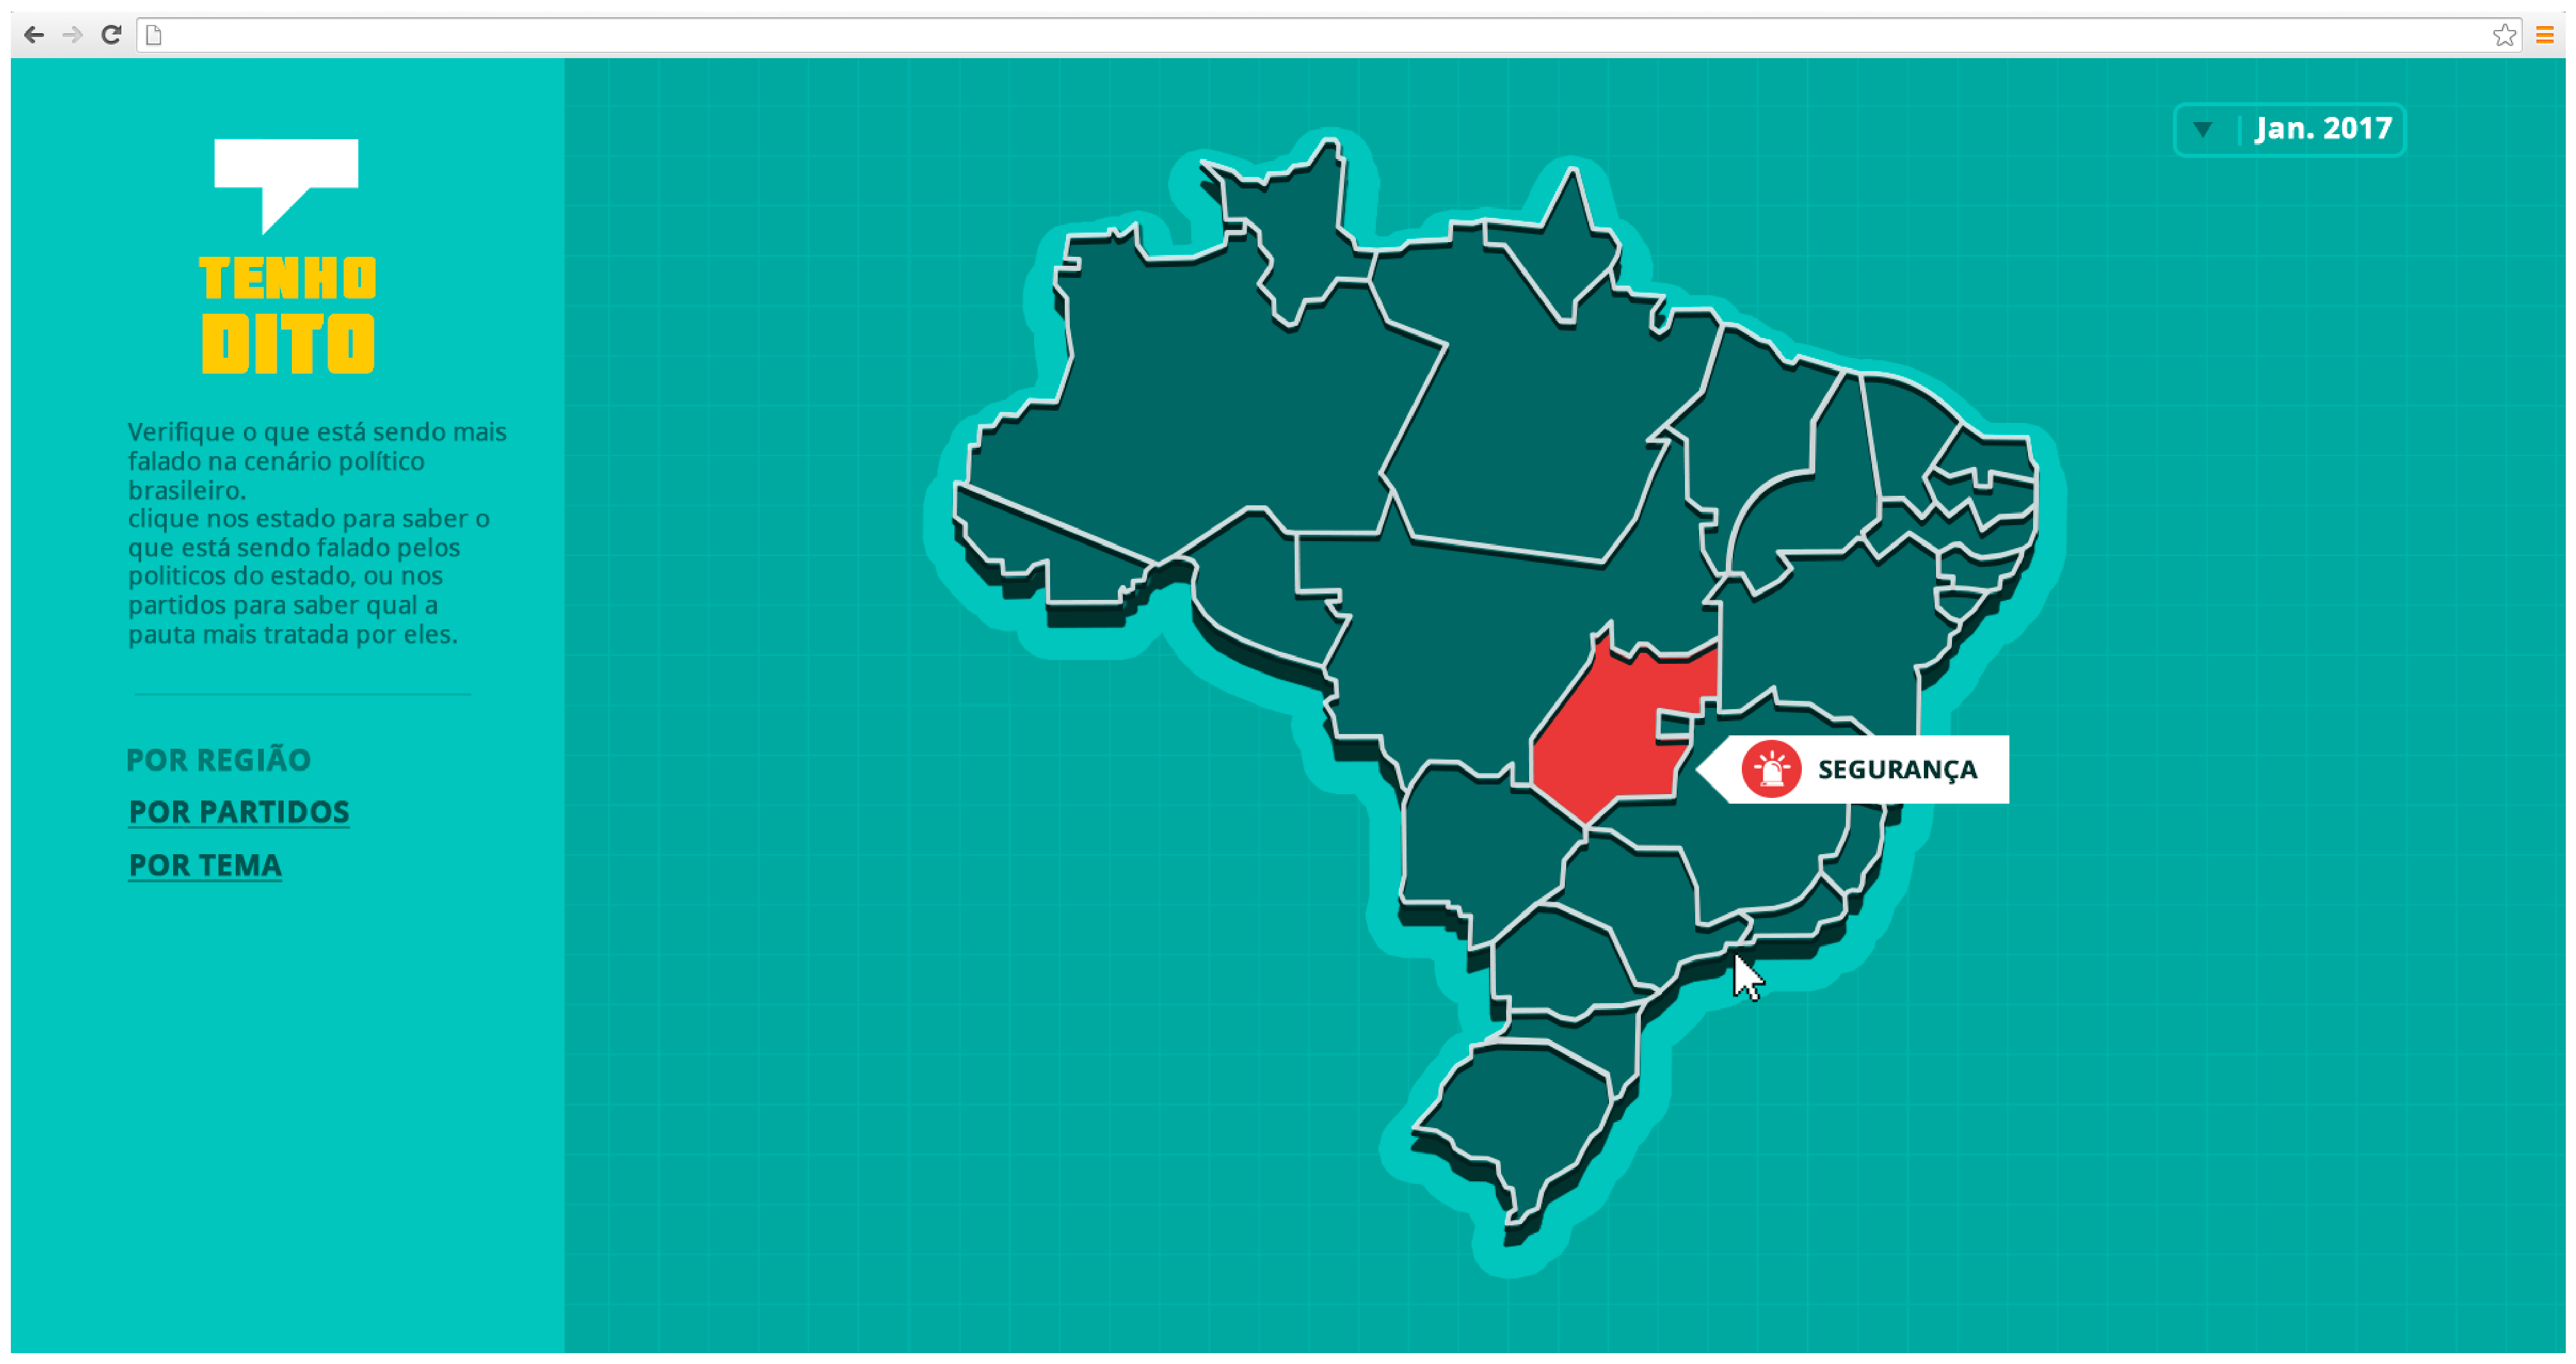
\includegraphics[scale=0.2]{figuras/tenhodito1.eps}
  \caption{Tela inicial do Tenho Dito - Visualização por região}
  \label{tenhodito1}
\end{figure}

Seguindo a abordagem por temas, ao clicar em um estado, o usuário é direcionado a outra página (figura \ref{tenhodito2}), onde encontra um gráfico de bolhas, detalhando os temas abordados pelos parlamentares do estado. Quanto maior a bolha, mais o tema foi abordado. Além disso, também são listados todos os deputados que representam aquele estado, juntamente com sua foto, partido e o tema predominante em seus discursos e proposições. Ainda não foram definidas as interações com o gráfico de bolhas.

\begin{figure}[h]
  \centering
  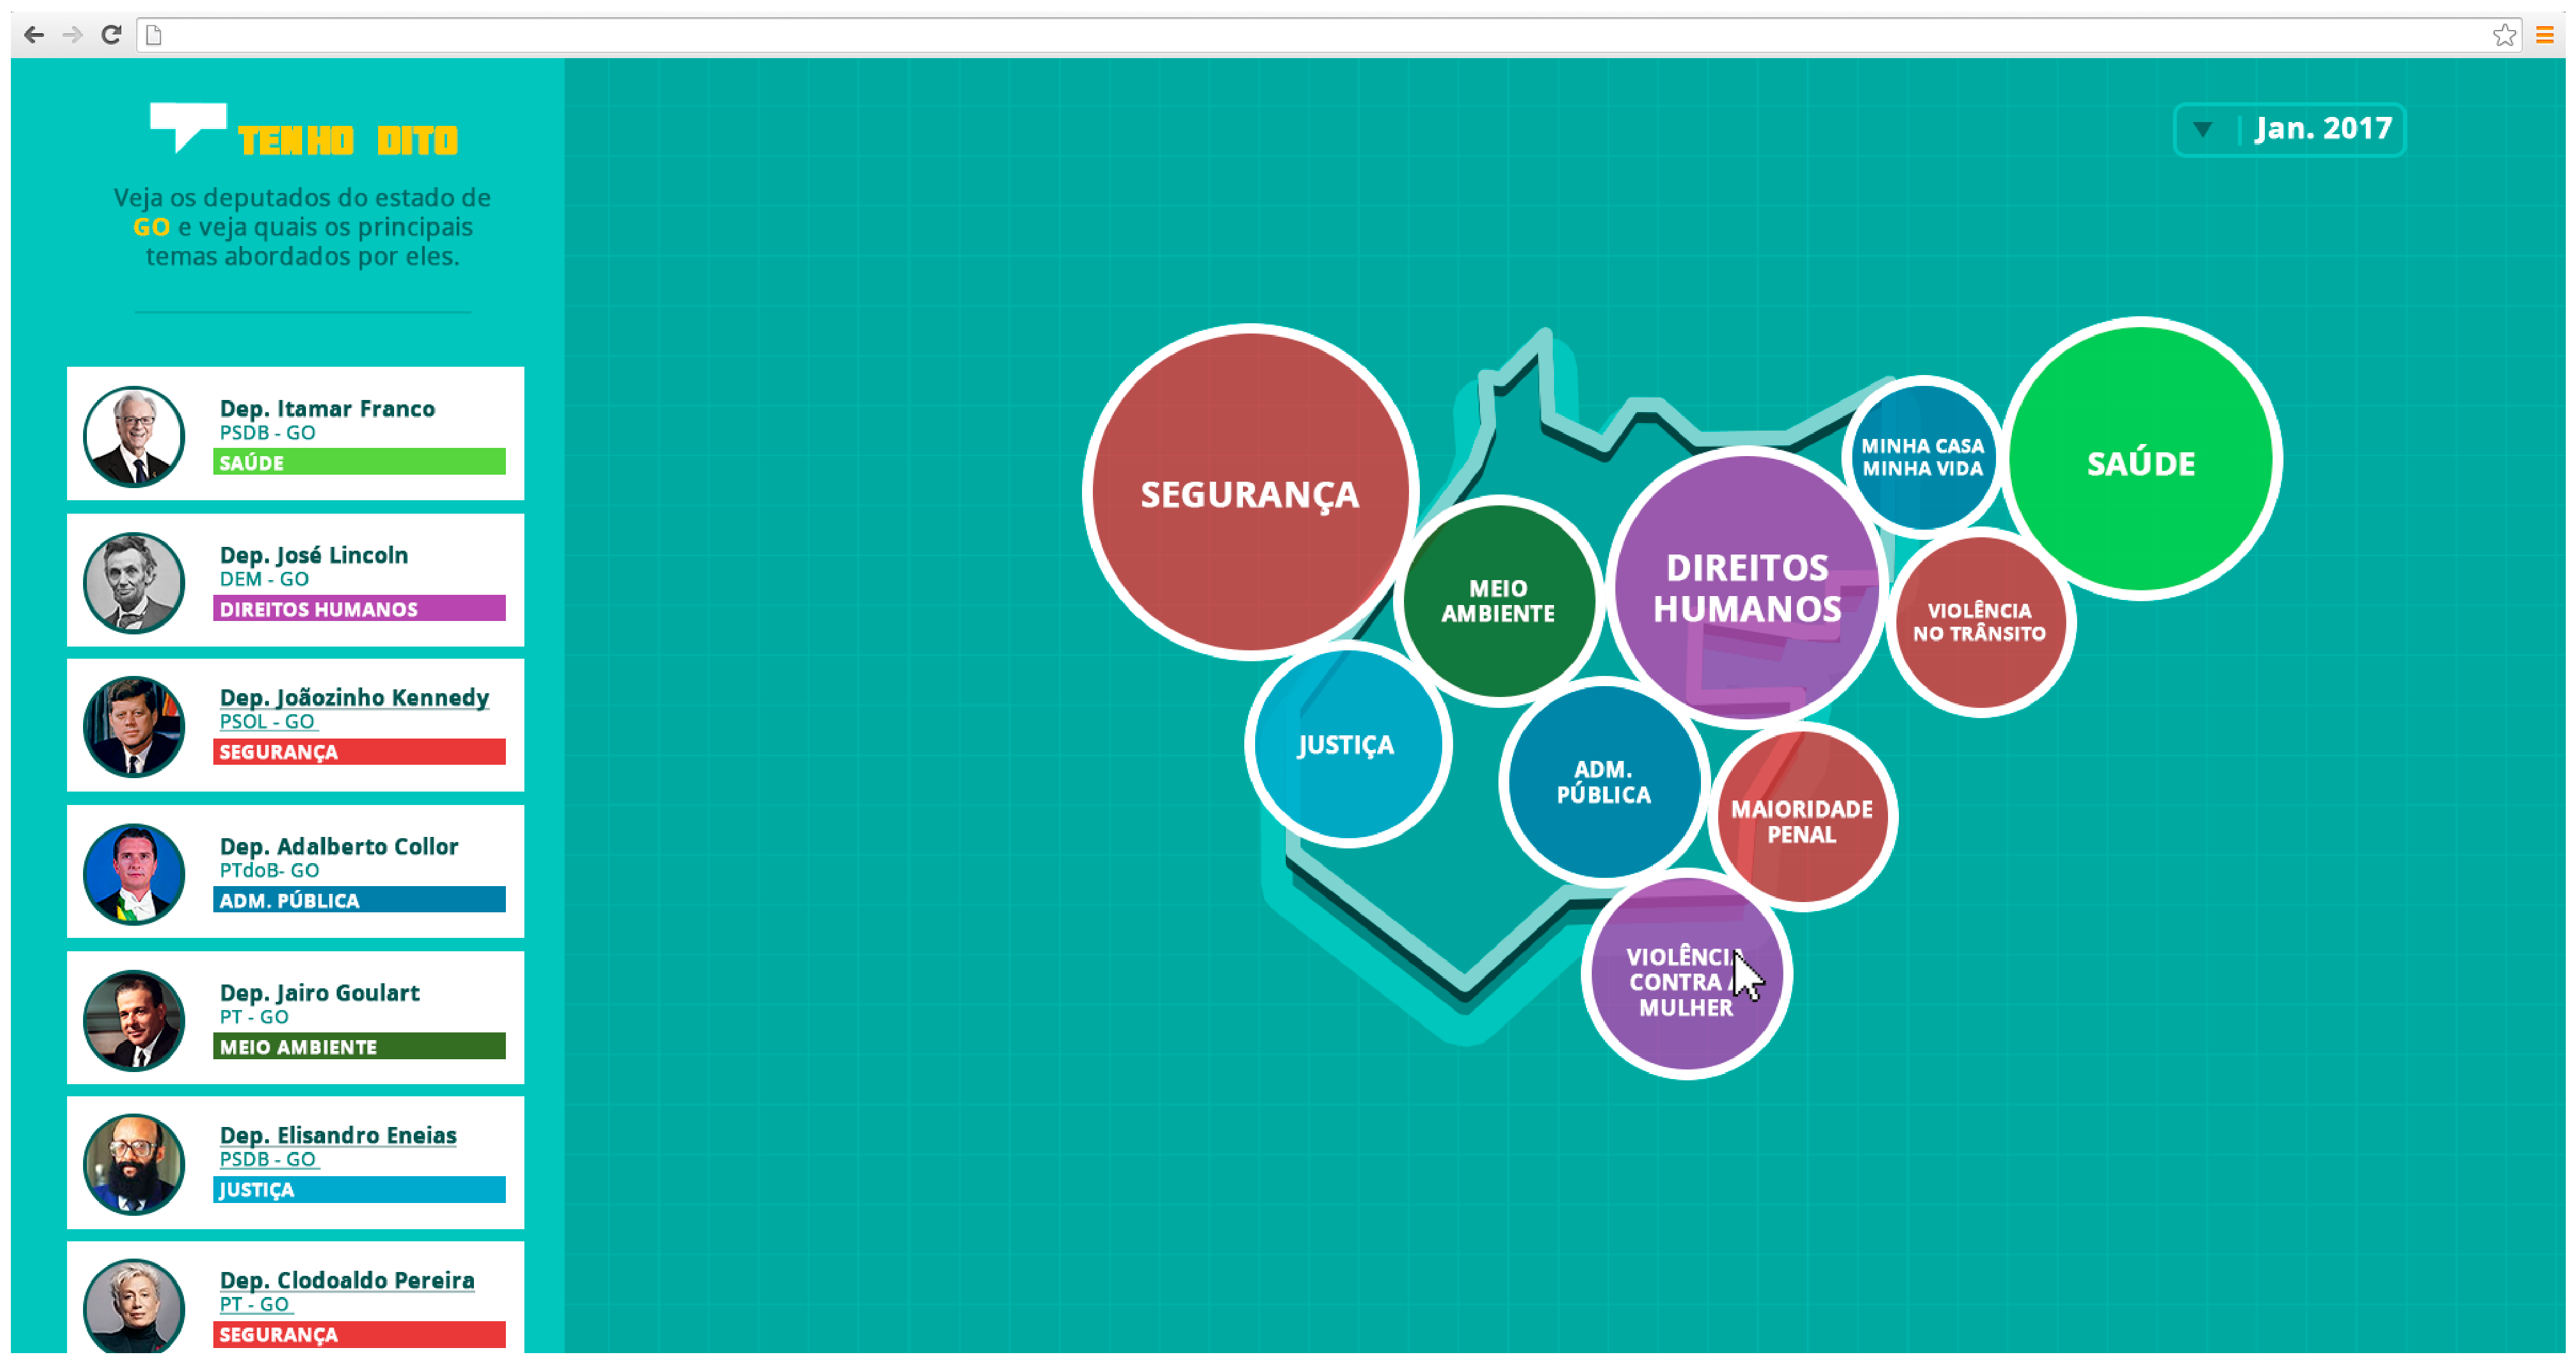
\includegraphics[scale=0.2]{figuras/tenhodito2.eps}
  \caption{Visualização detalhada dos temas, por região}
  \label{tenhodito2}
\end{figure}

O usuário também poderá selecionar um deputado específico e visualizar o seu perfil. Na tela de perfil do deputado (figura \ref{tenhodito3}), são exibidas as informações do deputado e também a quantidade de proposições e discursos analisados. Logo abaixo, será mostrado, dinâmica e randomicamente, trechos de discursos ou proposições e sua classificação. Além disso, serão listados todos os temas e a quantidade de discursos e proposições (por meio de gráfico de barras), com o objetivo de realizar uma comparação entre o que é mais dito pelo deputado e o que é mais proposto.

\begin{figure}[h]
  \centering
  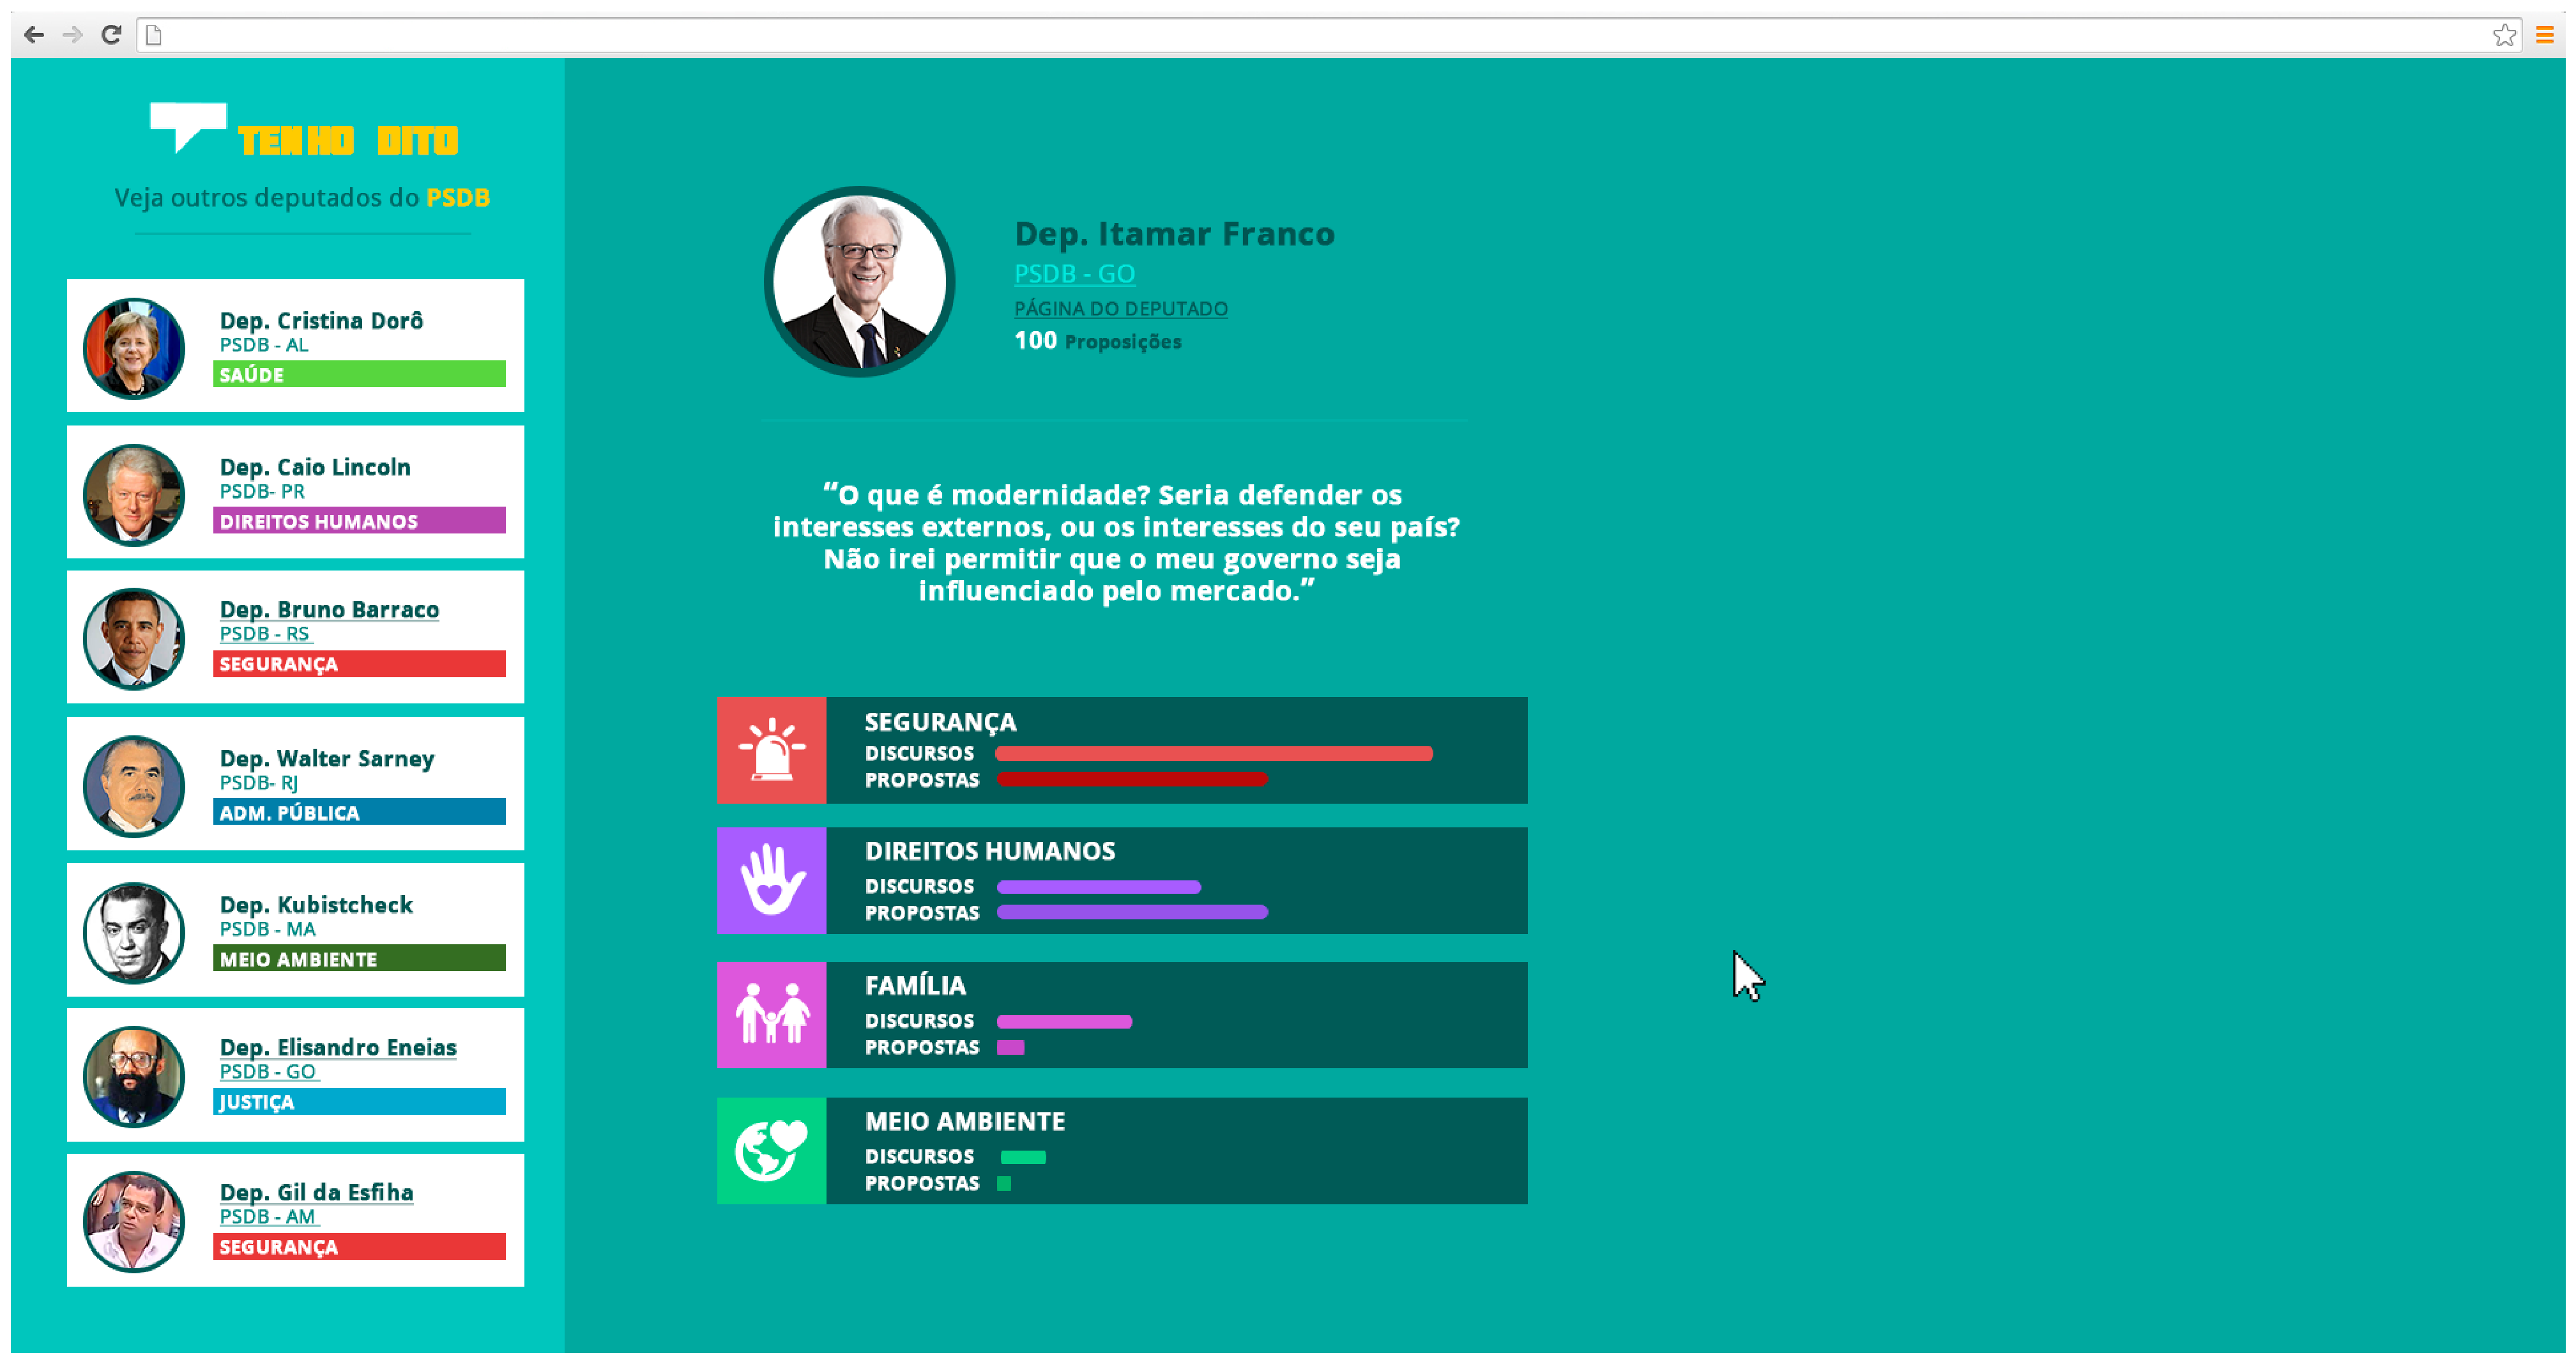
\includegraphics[scale=0.2]{figuras/tenhodito3.eps}
  \caption{Página de perfil do deputado}
  \label{tenhodito3}
\end{figure}

Quando o usuário clicar na opção de visualização por partidos, será exibida uma lista com os atuais partidos com representação na Câmara dos Deputados (figura \ref{tenhodito4}). O sitema possibilitará três tipos de ordenação: por tamanho (quantidade de deputados por partido), por ordem alfabética ou por tema. Nessa tela, também serão exibidos os temas mais abordados pelos partidos, através dos seus membros. Caso o partido tenho mais deputados cujo tema mais abordado em seus discursos e proposições é ``segurança'', por exemplo, o tema atribuído ao partido será ``segurança''.

\begin{figure}[h]
  \centering
  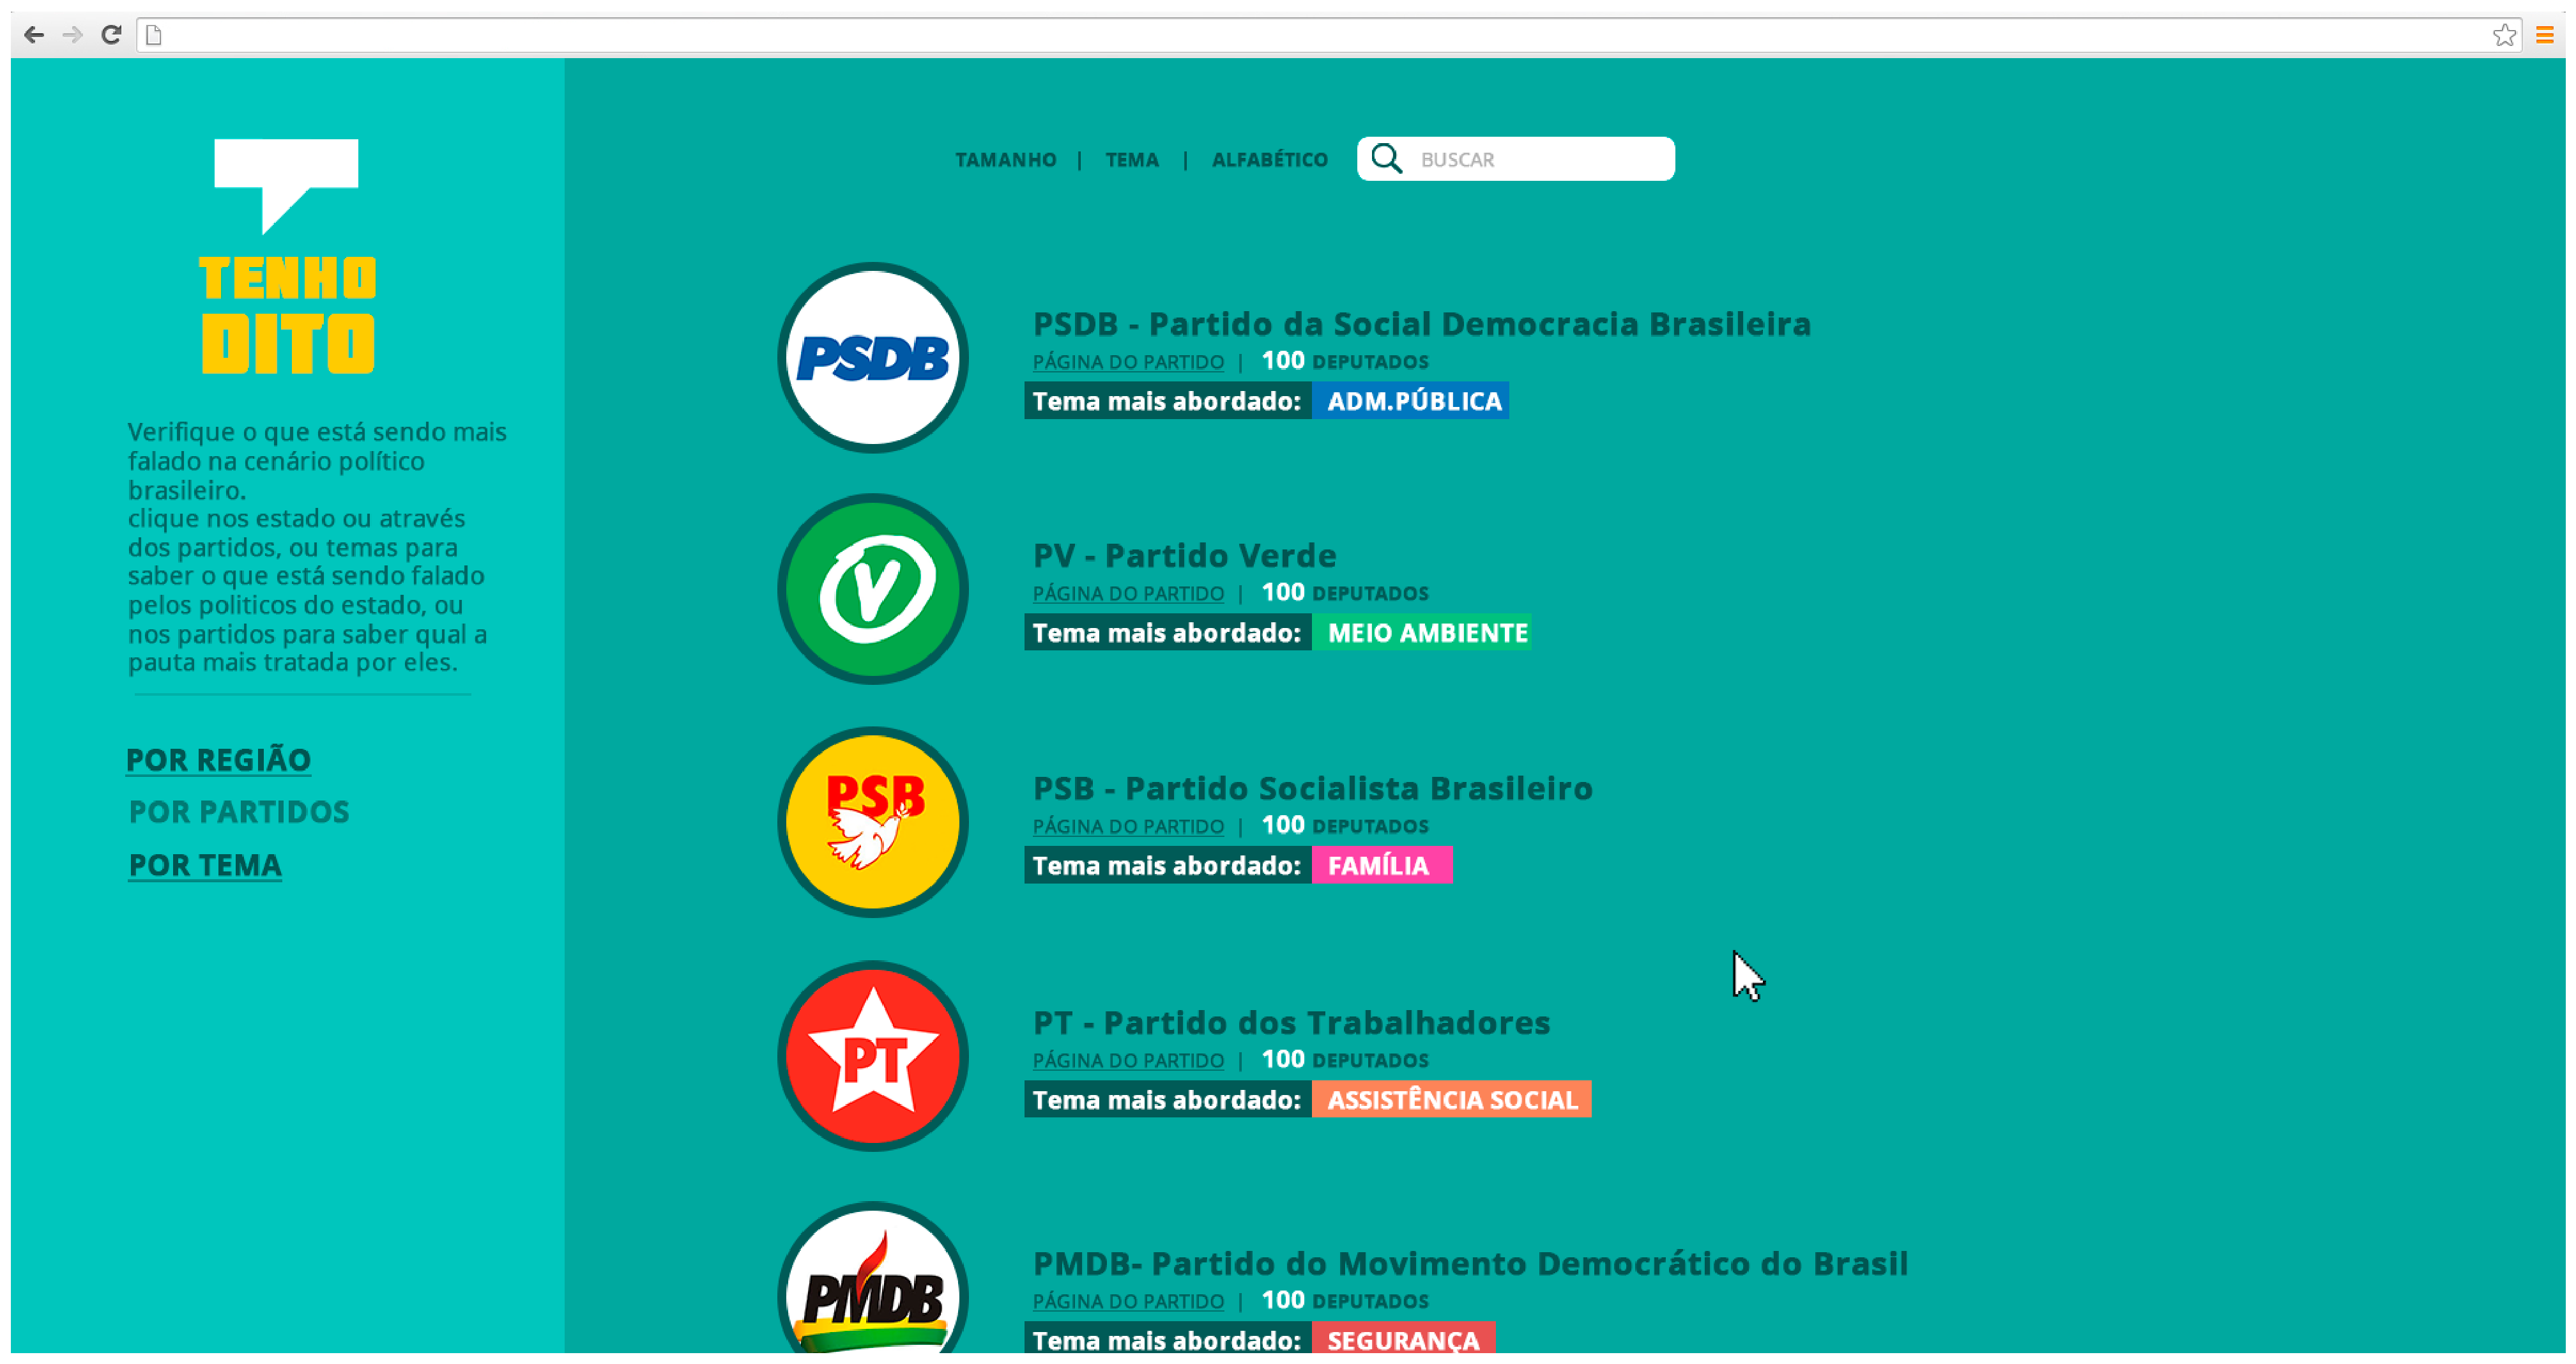
\includegraphics[scale=0.2]{figuras/tenhodito4.eps}
  \caption{Listagem dos partidos com representação na Câmara dos Deputados}
  \label{tenhodito4}
\end{figure}

O usuário poderá, assim como na abordagem por estado, escolher um partido para detalhar os temas abordados e, da mesma forma, é exibido um gráfico de bolhas com os temas abordados pelos deputados desse partido. Ao lado são mostrados todos os deputados do partido, independente do seu estado, ao clicar em algum deles o usuário é direcionado à pagina de perfil dele.

\begin{figure}[h]
  \centering
  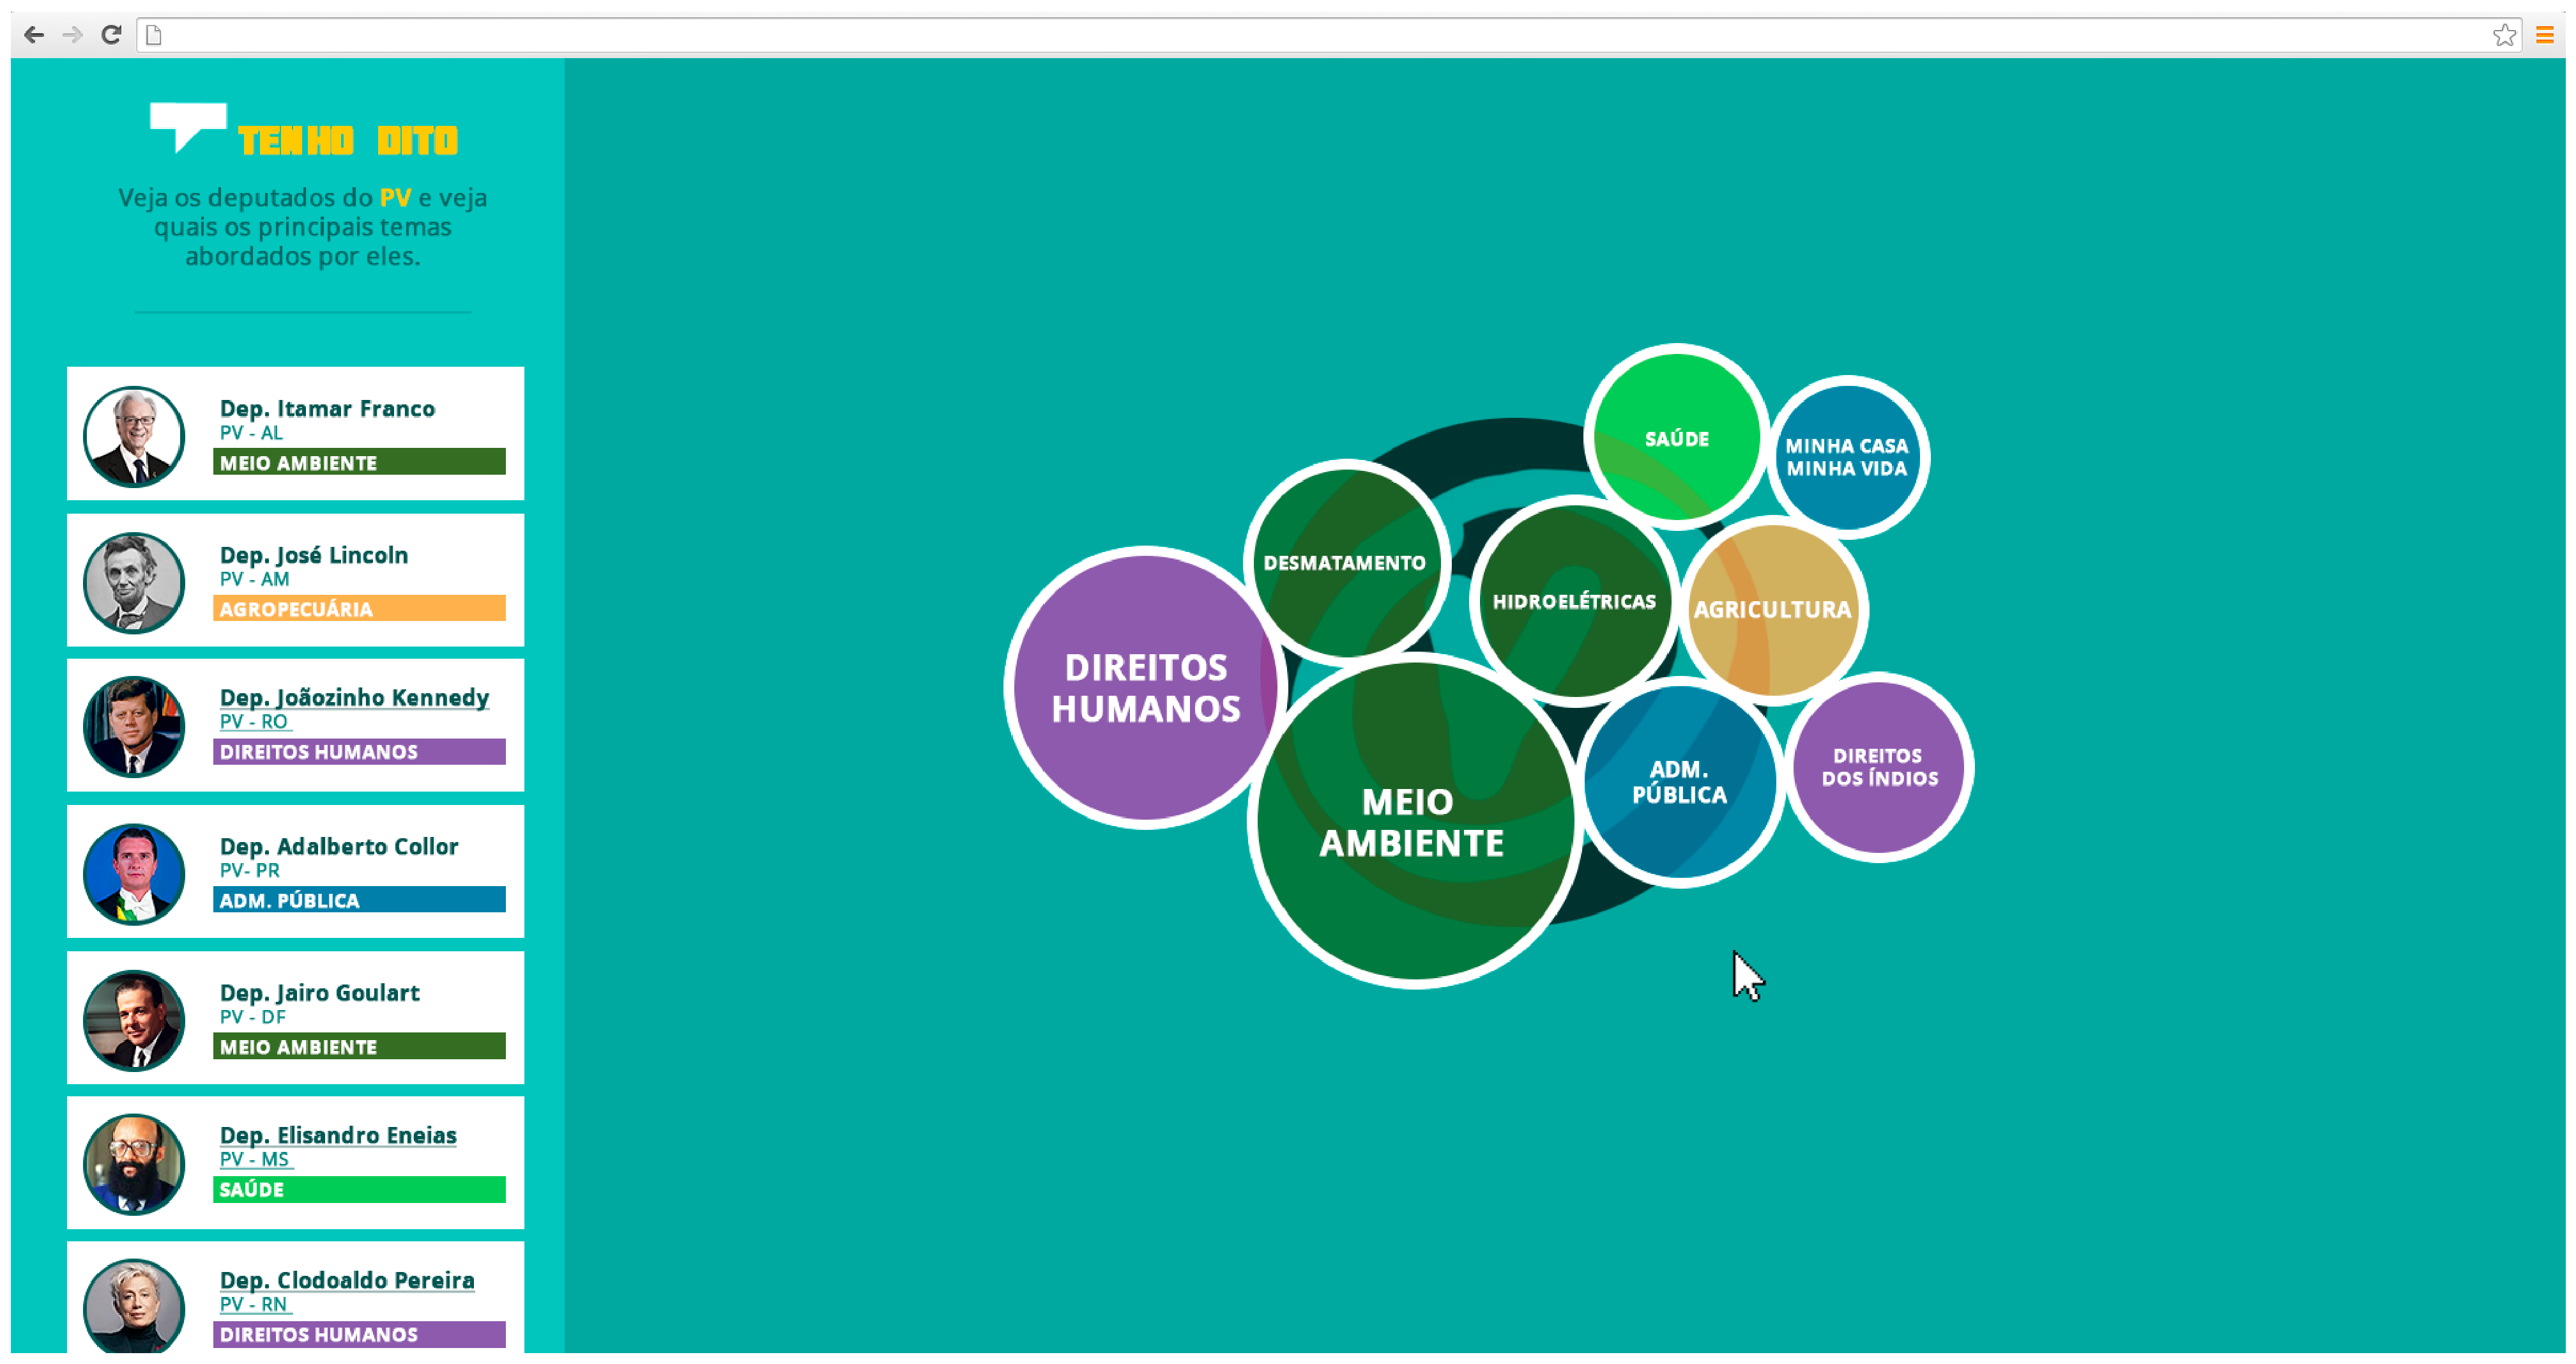
\includegraphics[scale=0.2]{figuras/tenhodito5.eps}
  \caption{Visualização detalhada dos temas, por partido}
  \label{tenhodito5}
\end{figure}

\chapter{\textit{Webservice} da Câmara dos Deputados}
\label{estrutura-webservice}

O \textit{webservice} atual (\textit{SOAP}) possui um total de 28 \textit{endpoints}, onde 5 são relacionados aos deputados, 9 aos órgãos, 9 às proposições e 5 às sessões e reuniões. A seguir descrevemos os \textit{endpoints} utilizados.

Os \textit{endpoints} que fornecem dados de deputados são:
\begin{itemize}
    \item \textbf{ObterDeputados:} retorna os deputados em exercício na Câmara dos Deputados
    \item \textbf{ObterDetalhesDeputado:} retorna detalhes dos deputados com histórico de participação em comissões, períodos de exercício, filiações partidárias e lideranças.
    \item \textbf{ObterLideresBancadas:} retorna os deputados líderes e vice-líderes em exercício das bancadas dos partidos
    \item \textbf{ObterPartidosCD:} retorna os partidos com representação na Câmara dos Deputados
    \item \textbf{ObterPartidosBlocoCD:} retorna os blocos parlamentares na Câmara dos Deputados.
\end{itemize}

Os \textit{endpoints} que fornecem dados de órgãos legislativos são:

\begin{itemize}
    \item \textbf{ListarCargosOrgaosLegislativosCD:} retorna a lista dos tipos de cargo para os órgãos legislativos da Câmara dos Deputados (ex: presidente, primeiro-secretário, etc)
    \item \textbf{ListarTiposOrgaos:} retorna a lista dos tipos de órgãos que participam do processo legislativo na Câmara dos Deputados
    \item \textbf{ObterAndamento:} retorna o andamento de uma proposição pelos órgãos internos da Câmara a partir de uma data específica
    \item \textbf{ObterEmendasSubstitutivoRedacaoFinal:} retorna as emendas, substitutivos e redações finais de uma determinada proposição
    \item \textbf{ObterIntegraComissoesRelator:} retorna os dados de relatores e pareces, e o link para a íntegra de uma determinada proposição
    \item \textbf{ObterMembrosOrgao:} retorna os parlamentares membros de uma determinada comissão
    \item \textbf{ObterOrgaos:} retorna a lista de órgãos legislativos da Câmara dos Deputados (comissões, Mesa Diretora, conselhos, etc.)
    \item \textbf{ObterPauta:} retorna as pautas das reuniões de comissões e das sessões plenárias realizadas em um determinado período
    \item \textbf{ObterRegimeTramitacaoDespacho:} retorna os dados do último despacho da proposição
\end{itemize}

Os \textit{endpoints} que fornecem dados de proposições são:

\begin{itemize}
    \item \textbf{ListarProposicoes:} retorna a lista de proposições que satisfaçam os critérios estabelecidos
    \item \textbf{ListarSiglasTipoProposicao:} retorna a lista de siglas de proposições
    \item \textbf{ListarSituacoesProposicao:} retorna a lista de situações para proposições
    \item \textbf{ListarTiposAutores:} retorna a lista de tipos de autores das proposições
    \item \textbf{ObterProposicao:} retorna os dados de uma determinada proposição a partir do tipo, número e ano
    \item \textbf{ObterProposicaoPorID:} retorna os dados de uma determinada proposição a partir do seu ID
    \item \textbf{ObterVotacaoProposicao:} retorna os votos dos deputados a uma determinada proposição em votações ocorridas no Plenário da Câmara dos Deputados
    \item \textbf{ListarProposicoesVotadasEmPlenario:} retorna todas as proposições votadas em plenário num determinado período
    \item \textbf{listarProposicoesTramitadasNoPeriodo:} retorna uma lista de proposições movimentadas em determinado período.
\end{itemize}

Os \textit{endpoints} que fornecem dados de sessões e reuniões são:

\begin{itemize}
    \item \textbf{ListarDiscursosPlenario:} retorna a lista dos deputados que proferiam discurso no Plenário da Cãmara dos Deputados em um determinado período.
    \item \textbf{ListarPresencasDia:} retorna a lista de presença de deputado em um determinado dia.
    \item \textbf{ListarPresencasParlamentar:} retorna as presenças de um deputado em um determinado período.
    \item \textbf{ListarSituacoesReuniaoSessao:} retorna a lista de situações para as reuniões de comissão e sessões plenárias da Câmara dos Deputados
    \item \textbf{ObterInteiroTeorDiscursosPlenario:} retorna o inteiro teor do discurso proferido no Plenário.
\end{itemize}

\chapter{Treinamento Inicial dos Classificadores}
\label{conjunto-palavras}

Para realizar o treinamento inicial dos classificadores \textit{naive} Bayes, é necessário fornecer um texto inicial e a sua classificação. Esse apêndice descreve os textos usados nesse trabalho para cada classificação.

\section{Classificação de Conteúdo Útil/Não-útil}

Para a classificação de ``conteúdo útil'' e ``conteúdo não-útil'', foram utilizadas os seguintes conjuntos de palavras iniciais:

\begin{itemize}
    \item \textbf{Conteúdo não-útil:} ``agradecimento agradeço muito obrigado v.exa. digníssimo nobre deputado amigo peço registro pela ordem pedir um aparte mérito emendas votado sessão comissão protocolo regimento pronunciamento divulgação''
    \item \textbf{Conteúdo útil:} ``educação universidade estudante professor ensino escola educador saúde médicos hospitais sus remédios atendimento hospitalar tratamento leitos religião templo igreja deus bíblia fé jesus segurança polícia crime violência punição arma contrabando ditadura militar golpe 31 de março tortura censura mulher aborto feminicídio feminismo feminista maria da penha petrobras pré-sal refinamento gasolina álcool combustível petrolão corrupção ministério público agu lava-jato mensalão impeachment crime de responsabilidade agronegócio agricultura agrícolas soja lavoura rural indústria desendustrialização empregos competitividade direitos humanos minorias tortura tráfego de pessoas trabalho escravo''
\end{itemize}

\section{Classificação Temática}

Para a classificação temática, os temas escolhidos e seus respectivos conjuntos de palavras utilizados foram:

\begin{itemize}
    \item \textbf{Agropecuária:} ``agropecuária fertilizantes agronegócio abate suínos ovos cabeças bovinos frangos exportação carne animal milho ração aviária laranja safra frutos pomares laranjeiras fazenda pés produzir hectares quilos fruta  produtor orgânico consumidor toneladas  embrapa bezerros pecuária veterinária filhotes sementes agro produção água sol área degradação produtor café importação agrícola pescador alimento alimentação açúcar ibge fertilizante lavouras grão bovino soja etanol frutos rural''
    \item \textbf{Saúde:} ``saúde médico doença vírus zika pesquisa paciente estudo mosquito epidemia chikungunya tratamento procedimento tremor causa gêmeos dengue transmissão cubano bebês cirurgia cientista risco sintomas dor ultrassom dr aegypt ovário microcefalia gravidez sistema imune imunológico drogas fertilização febre diagnóstico renal sangue insuficiente insuficiência cérebro idade nascimento hipotálamo morte dna corpo cardio muscular vacina''
    \item \textbf{Esporte:} ``esporte jogo jogador clube time contrato treino mundial atleta surf futebol disputa penalidade compo estádio ataque atacante bola goleiro treinador seleção técnico campeonato gol pontuação futsal vitória perde perdedor lutador torcedor torcida rival diretor falta conquista prorrogação empate surfista assistência ufc''
    \item \textbf{Educação:} ``educação estudo ensino escola médio prova enem universidade faculdade matemática avaliação aluno curso pesquisa inep exame pública mec professor redação criança texto reforma currículo curricular campus leitura literatura desempenho formação qualidade disciplina fies superior analfabeto analfabetismo português física química geometria''
    \item \textbf{Ciência e Tecnologia:} ``ciência tecnologia novidades empresa startup smart serviço smartphone consumidor produto google aparelho samsung celular internet inteligência artificial desenvolvimento dispositivo lançamento  aplicativo inovar inovação sony conectar conectado comunicação 3g 4g 5g iphone sistema telecomunicações satélite design científico artigo computador tráfego eletrônico apple whatsapp televisão tv telefone avanço espacial''
    \item \textbf{Economia:} ``economia trabalho crédito compra banco bilhões milhões vendas contas inflação consumidor juros queda crise taxa resultado econômico gasto pagamento valor financeiro investimento dinheiro índice comércio empresa desemprego fgts limite emprego cartão varejo déficite fundo recessão recuo salário lojista tesouro fiscal inadimplente recurso dólar euro moeda bolsa endividado projeções crescimento capital ações negócios''
    \item \textbf{Política:} ``política deputado congresso pt partido estado união reforma lei legislatura legislação pec pmdb aprovar voto bancada população senado senador câmara deputado sindicato candidato candidatura mandato comissão ministério constituição eleição eleições delação judiciário votações prefeitura prefeito vereador assembleia procurador corrupção''
    \item \textbf{Meio Ambiente:} ``ambiente área água rio empresa desastres multa seca barragem furacão desmatamento floresta tropical ibama parque preservação região terra planeta poluição ambiental espécie animais plantas platações petróleo emissão gás chuva temporal sol clima temperatura estufa aquecimento global umidade terremoto planeta biodiversidade biologia mar oceano calor energia sustentável madeira reflorestamento tempestade niño florescimento hídrico climática''
    \item \textbf{Direitos Humanos:} ``direitos humanos mulher tortura violência morte justiça onu sexual vítima sexual adolescente presídio prevenção união negro branco segurança refugiado homens humanitario conflito sociedade racismo sexismo machismo machista feminismo feminista defensoria estupro jovens criança prostituição assassinato liberdade idoso inclusão social preconceito gay homossexual heterosexual lgbt lésbica bissexual travesti transexual transgênero impunidade imigrante''
    \item \textbf{Segurança:} ``segurança ataque polícia suspeito morte crime terror rebelde investigação civil federal guerra onu vítima invasão preso presídio assassinato bombardeio apreensão incidente defesa exército marinha aeronáutica prisão ameaça bomba testemunha promotor policial tragédia assalto protesto''
\end{itemize}


\end{apendicesenv}
